\section{Dynamic Ranking Computation}
\label{sec-incAlg}

Scholarly articles are dynamic and continuously growing, and it is impractical to recompute ranking from scratch once they get updated. In this section, we present an incremental algorithm for our ranking model \ensemblerank.


\subsection{Incremental Algorithm Framework}
\label{subsec-inc-alg}




Our incremental algorithm \incensemble incrementally computes the popularity and prestige of scholarly articles.
We consider that an update $\Delta$ = $\Delta V\cup\Delta E$ is added to a   (citation or venue) graph $G(V, E)$,
and the resulting graph is $G^+(V\cup\Delta V, E\cup\Delta E)$, where
$\Delta V$ is a set of nodes with $\Delta V\cap V = \emptyset$, and $\Delta E$ is a set of directed edges on $\Delta V$ and from $\Delta V$ to $V$ only, as article citation relationships obey a natural temporal order, \ie an article only cites those published earlier, and it is rare for the mutual citations between two articles published in the same time.


\stitle{Incremental popularity computation}.
The popularity of venues and authors is computed along the same lines as their batch counterparts of algorithm \batensemble,
as almost all venues and authors are affected  by the definitions of the popularity of venues and authors.


As the popularity of articles is defined as the freshness sum of all their citations, it is convenient to maintain in a dynamic scenario. Consider an updated citation graph $G^{c,+}(V^c\cup\Delta V^c, E^c\cup\Delta E^c)$ of $G^c(V^c, E^c)$, and the updated popularity $Pop_{c}^+(v)$ can be computed as:

\vspace{-1ex}
\begin{small}
\begin{equation}\label{eq-inc-pop}
Pop_c^+(v) = Pop_c(v) {e^{\sigma (T^+_0-T_0)}} + \sum_{(u,v)\in \Delta E^c} {e^{\sigma (T^+_0-T_u)}},
\end{equation}
\end{small}
\noindent
where $Pop_c(v)$ (resp. $Pop_c^+(v)$) is the popularity of node $v$ on $G^c$ (resp. $G^{c,+}$), and
 $T_0$ (resp. $T^+_0$) is the current time in $G^c$ (resp. $G^{c,+}$).
%
By Eq.~(\ref{eq-inc-pop}), it is easy to see that it takes $O($ $|V^c|+|\Delta V^c|+|\Delta E^c|)$ time to update the popularity.
%This further shows that Eq.~(\ref{eq-inc-pop}) is a desired solution for popularity maintenance.



\stitle{Incremental prestige computation}.
The prestige of authors is computed along the same lines as the batch algorithm \batensemble,
as almost all authors are affected  by the definition of the prestige of authors.
%
For articles and venues, we propose an incremental algorithm to maintain their prestige.



%We first present the incremental  prestige computation. Again, it differs for the prestige of articles and venues in a specific year and the one of authors. We finally present the complete incremental algorithm \incensemble, which is similar to the batch algorithm \batensemble, except that (1) it uses algorithm \inctwprscc to incrementally compute the prestige of articles and venues, and (2) it incrementally computes the popularity of articles based on Eq.~(\ref{eq-inc-pop}).




\subsection{Incremental TWPageRank Computation}
\label{subsec-incTWPageRank-computation}

%\subsubsection{Prestige of articles and venues in a specific year}
%\label{subsubsec-incprs-CV}
%\subsubtitle{Prestige of articles and venues in a specific year}.
%We expand $M$ and $PR$ to the same sizes as $M^+$ and $PR^+$, respectively, by filling zeros, and let $\Delta M=M^+ - M$ and $\Delta PR = PR^+ - PR$.




Consider a citation or venue graph $G(V, E)$, its TWPageRank vector $PR$ and the topological order $O$ of its block-wise graph. Given an update $\Delta$ = $\Delta V\cup\Delta E$ to $G$, the incremental prestige computation for articles and venues in a specific year is to compute the TWPageRank vector $PR^+$ on the updated graph $G^+(V\cup\Delta V, E\cup\Delta E)$.


\stitle{Auxiliary data structure maintenance}.
Two auxiliary data structures in the batch algorithm~\twprscc need to be maintained : (a) on the block-wise graph,  a mapping that, given a node of graph $G$, returns the index of the \scc to which it belongs, and (b) the topological order of the nodes in the block-wise graph.
%
Observe that these auxiliary data structures can be easily maintained as follows.

%the idea is to divide $G$ into affected and unaffected areas such that TWPageRank scores of nodes in affected and unaffected areas are updated accordingly.


\sstab(1) The block-wise graph of $G^+$ needs to be computed, whose \sccs consist of the \sccs in $G$ and \sccs in the induced subgraph $G^+[\Delta V]$, as  the edges of $\Delta E$ are  on nodes in $\Delta V$ and from $\Delta V$  to $V$ only. Hence, only those new \sccs in $G^+[\Delta V]$ need to be computed.

\sstab(2) The updated topological order $O^+=\Delta O/O$, where $\Delta O$ is the topological order of the block-wise graph of induced subgraph $G^+[\Delta V]$. Hence, only $\Delta O$ needs to be computed. One can easily verify the following.


\begin{prop} \label{lemma-inc-topo}
 $O^+=\Delta O/O$ is indeed a valid topological order of the block-wise graph of $G^+$.
\end{prop}

\begin{proofSketch}
We prove that for each edge $(u,v)$ in the block-wise graph of $G^+$, node $u$ comes before $v$ in $O^+$, and the conclusion follows by the definition of topological order.
\end{proofSketch}

\eat{
\begin{proof}
Let $E'_c$ denote the set of cross edges from $V'_\Delta$ to $V'$.
It suffices to show that for each $(u,v)\in E'\cup E'_\Delta \cup E'_c$, $u$ comes before $v$ in $O^+$,
which obviously holds (1) for  $E'\cup E'_\Delta$ as $O$ and $\Delta O$ are topological orders of $G'$ and $G'_\Delta$, respectively, and (2) for $E_{c}'$ as nodes in $G'_\Delta$ come before nodes in $G'$.
\end{proof}
} %%%%%%%%%% for eat


%%%%%%%%%%%%%%%%%%%%%Algorithm
\begin{figure}[tb!]
%\vspace{2ex}
\begin{center}
{\small
\begin{minipage}{3.36in}
\myhrule \vspace{-1.5ex}
\mat{0ex}{
%%%%%%%%%%%%%%%%%%%
{\sl Input:\/} \= An update $\Delta$ = $\Delta V\cup\Delta E$, TWPageRank vector $PR$ of $G$,\\
\hspace{5ex}   and the  topological order $O$ of the block-wise graph $G'$.\\
{\sl Output:\/} TWPageRank vector $PR^+$ of the updated graph $G^+$. \\
\\
\bcc \hspace{1.5ex}\=  $G_C'$ := the block-wise graph of $G_C$; \\
%\ \  $E_{CB}'$ := edges from $G_C'$ to $G'$\\
\icc\> $\Delta O$ := topological order of $G_C'$; \ \ $O^+$ := $\Delta O/O$; \\
\icc\> label \sccs of $G_C$ as $C$ and \sccs of $G$ with outgoing edges \\ \hspace{2.5ex}  having  weight changes as $B$,  the remaining \sccs of $G$ as $A$\\
\icc\>  \For each node $v'$ following $O^+$ \Do\\
\icc\>\hspace{2.5ex}\= $scc$ := the corresponding \scc of $v'$; \\
%\icc\>\>\If impact weight of $(v,w)$ is changed where $v\in scc$ \Then \\
%\icc\>\>\hspace{3ex}\= label $scc$ as $B$;\\
%\icc\>\>\> label SCC $w'$ as $B$ such that $(v',w')\in E'$; \\
\icc\>\> \If $scc$ is labeled as $C$ \Then \\
\icc\>\>\hspace{3ex}\= update $PR^+(v)$ ($v\in scc$) following algorithm~\twprscc; \\
\icc\>\>\> label \scc $w'$ as $B$ with $w'\in G'$ and $(v', w')\in E^+{'}$;\\
\icc\>\> \Else \If $scc$ is labeled as $B$ \Then \\
\icc\>\>\> update $PR^+(v)$ where $v\in scc$ with Eq.~(\ref{eq-inc-prscc}) until the \\ \hspace{8ex}  sum of TWPageRank score changes is less than $\epsilon\cdot \frac{|scc|}{|V^+|}$; \\
\icc\>\>\> label \scc $w'$ as $B$ with $(v',w')\in E'$;\\
\icc\>\> \Else $PR^+(v)$:=$PR(v)\cdot {n}/{n^+}$ where $v\in scc$; \\
\icc\> \Return $PR^+$.
}
\vspace{-2.5ex} \myhrule
\end{minipage}
}
\end{center}
\vspace{-1ex}
\caption{\small Algorithm~\inctwprscc for incremental TWPageRank} \label{alg-inctwprscc}
\vspace{-3ex}
\end{figure}
%%%%%%%%%%%%Algorithm

%%% affected/unaffected division
\stitle{Analyses of affected and unaffected areas}.
The TWPageRank vector $PR$ of graph $G$ is mainly affected in two ways.



\sstab(1) Let $V_{B,1}\subseteq V$ be the set of nodes reachable from the newly added nodes $\Delta V$, $V_{B,2}\subseteq V$ be the set of nodes with outgoing edges having weight changes, and $V_{B,3}\subseteq V$ be the set of nodes reachable from  $V_{B,2}$.
%
Then $V_B=V_{B,1}\cup V_{B,2}\cup V_{B,3}$ is obviously the set of nodes in $G$ affected by the update $\Delta$.
%
TWPageRank scores on $V_B$ are re-iterated as follows, where notations with superscript `$+$' are defined on  $G^+$.
%using the existing TWPageRank vector scaled with constant ${n}/{n^+}$.

\vspace{-2ex}
\begin{scriptsize}
\begin{equation}\label{eq-inc-prscc}
\begin{split}
PR^+(v) \ = \ &  d \sum_{(u,v)\in E^+_i} M^+_{u,v} PR^+(u) + d \sum_{(u,v)\in E^+_a} M^+_{u,v} PR^+(u)  \\
 + \frac{n}{n^+} \Big( PR(v) &  - d \sum_{(u,v)\in E_i} M_{u,v} PR(u) - d\sum_{(u,v)\in E_a} M_{u,v} PR(u)\Big).
\end{split}
\end{equation}
\vspace{-2ex}
\end{scriptsize}


\sstab(2) Let $V_A = V\setminus V_B$. Since nodes in $V_A$ are not reachable from newly added or affected nodes, $V_A$ is essentially not affected by the update $\Delta$. And TWPageRank scores on $V_A$ only need to scale with constant ${n}/{n^+}$.

Let $G_A=(V_A,E_A)$, $G_B=(V_B,E_B)$ and $G_C=(V_C,E_C)$, respectively, and
let $E_{AB}$ and $E_{CB}$  be the sets of edges from $G_A$ to $G_B$ and from $G_C$ to $G_B$, respectively.
In this way, graph $G^+$ is divided into subgraphs $\{G_A$, $G_B$, $G_C\}$ and edge sets $\{E_{AB}, E_{CB}\}$.
%
We then have $G_C$ = $G^+[\Delta V]$, $\Delta E$ = $E_C\cup E_{CB}$, $V$ = $V_A\cup V_B$ and $E$ = $E_A\cup E_B\cup E_{AB}$.



\stitle{Incremental algorithm \inctwprscc}. We now present our incremental algorithm for TWPageRank, shown in Fig.~\ref{alg-inctwprscc}.


It takes as input an update $\Delta$ and the previous results on the original graph $G(V, E)$, and returns the TWPageRank vector of the updated graph $G^+$. It first incrementally computes the topological order $O^+$
%by concatenating the topological orders of $G_C'$ and $G'$
(lines 1--2). %Note that $G_C'$ is the same to $G'_\Delta$.
%
After that, it labels the newly added \sccs with $C$ and existing \sccs with $A$ or $B$, depending on whether the existing \sccs have weight changes on outgoing edges (line 3).
%
It then processes each \scc in the order $O^+$ such that the TWPageRank scores of nodes in each \scc are updated according to the labels (lines 4--12), and finally returns the TWPageRank vector (line 13).
%
%More specifically, the scores of nodes in SCCs labeled as $C$ and $B$ are updated the same to Algorithm~\twprscc, while the scores of nodes in SCCs labeled as $A$ are simply scaled.
%
%It is also easy to verify that nodes in SCCs labeled as $A$, $B$ and $V$ corresponding to $V_A$, $V_B$ and $V_C$.

When processing $V_B$ with Eq.~(\ref{eq-inc-prscc}), {\em edges in $E_{AB}$ can be skipped}  since $PR^+(u)={n}/{n^+}\cdot PR(u)$ for $u\in V_A$ and $M_{u,v}=M^+_{u,v}$ for $(u,v)\in E_{AB}$. Besides, we use ${n}/{n^+}\cdot PR$ as the initial vector. Both of them can speed up the computation.


\eat{
\begin{figure}[tb!]
\centering
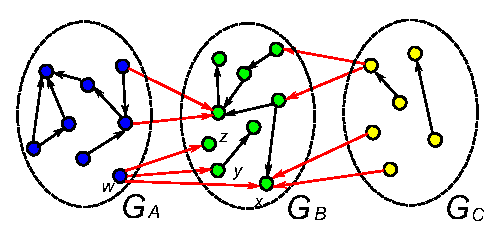
\includegraphics[scale=0.6]{fig/General_framework_peak_ABC.eps}
\vspace{-3ex}
\caption{\small An example of affected and unaffected areas}
\label{fig-inc-division}
\vspace{-3ex}
\end{figure}

\begin{example} \label{eg-layer-dag}
Figure~\ref{fig-inc-division} illustrates an example of affected and unaffected areas, in which subgraphs $G_A$, $G_B$ and $G_C$ are associated with node sets $V_A$, $V_B$ and $\Delta V$, respectively. Here the citation peak time of node $x$ is changed, which leads to the changes of the normalized weights of edges $(w,x)$, $(w,y)$ and $(w,z)$.
\end{example}
}


\begin{figure}[tb!]
\centering
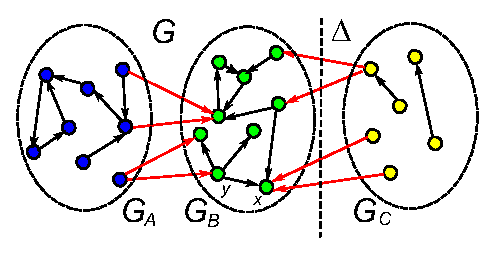
\includegraphics[scale=0.7]{fig/General_framework_peak.eps}
\vspace{-1ex}
\caption{\small An example of incremental TWPageRank computation}
\label{fig-inc-division}
\vspace{-3ex}
\end{figure}

\begin{example} \label{eg-layer-dag}
Figure~\ref{fig-inc-division} illustrates an example of incremental TWPageRank computation. Consider an update $\Delta$ on the original graph $G$.
%
It is obvious that the update $\Delta$ has no impacts on the SCCs of $G$, and $O^+$ defined earlier is a valid topological order of $G^+{'}$.
%
The original graph $G$ is then partitioned into affected and unaffected areas, and subgraphs $G_A$, $G_B$ and $G_C$ are associated with node sets $V_A$, $V_B$ and $\Delta V$, respectively. Here edge weight on $(y, x)$ changes due to the change of the citation peak time of node $x$, and, hence, node $y$ as well as all nodes reachable from $y$ are included in $G_B$.
%
When updating the TWPageRank scores, following $O^+$, scores of nodes in $G_C$, $G_B$ and $G_A$ are computed by iterations from scratch, by iterations with Eq.~(\ref{eq-inc-prscc}) using the existing TWPageRank vector and by scaling, respectively.
\end{example}

\vspace{-1ex}
\begin{theorem}
\label{lemma-subgraphA}
The TWPageRank vector $PR^+$ returned by~\inctwprscc converges such that $||PR^+-PR^{*}||_1 < \epsilon$, where $PR^{*}$ is the convergent TWPageRank vector.
\end{theorem}


\begin{proofSketch}
Assume a topological order $v_1'/\dots/v_{l}'$ of the block-wise graph $G^+{'}$ where $l=|O^+|$. It suffices to prove by induction that the sum of changes of $PR^+(v)$ ($v\in scc_k$) is no more than $\epsilon |scc_k|/|V^+|$ for $scc_k$ of $v_k'$ ($k\in [1,l]$).
%The conclusion follows combining Lemma~\ref{prop-prscc}
%(see \cite{SARank-full} for details).
\end{proofSketch}




Observe that (a) a topological order of $G'_C$ can be computed in $O(|V_C|+|E_C|+|E_{CB}|)$ time,
(b) updating the TWPageRank scores of nodes in subgraphs $G_B$ and $G_C$ costs $O(|V_B\cup V_C|+|E_{B,a}\cup E_{C,a}\cup E_{CB}|)+t^+|E_{B,i}\cup E_{C,i}|)$ time, and , finally, (c) updating the scores of nodes in $G_A$ costs $O(|V_A|)$ time. From these, the following holds.


\begin{prop} \label{lemma-inc-citation-comp}
Given an update $\Delta$ = $\Delta V\cup\Delta E$ of citation or venue graph $G(V,E)$, the TWPageRank vector of $G$ and the topological order of $G'$, algorithm \inctwprscc runs in $O(|V\cup \Delta V| + |E_B\cup E_C\cup E_{CB}| + t^+|E_{B,i}\cup E_{C,i}|)$ time.
\end{prop}



%Note that the incremental algorithm reduces the complexity of updating subgraph $A$ from $O(|E^c_A|)$ to $O(|V^c_A|)$. It is more effective when only a small number of articles are updates, resulting in $|V^c_A|>>|V^c_B|+|V^c_C|$ and updating subgraph $A$ occupies most of the computation.

By Propositions~\ref{prop-converg} \& \ref{lemma-inc-topo} and Theorem \ref{lemma-subgraphA}, one can easily verify the correctness of algorithm \inctwprscc.
%
Note that  a) algorithm \inctwprscc computes \sccs and derives the topological order based  on $\Delta$ only, instead of $G^{+}$,
b) it skips edges in $E_A\cup E_{AB}$ when updating the scores of nodes in $G_A$ and $G_B$, and
c) the number $t^+$ is very likely smaller than the number $t$ of \twprscc when updating scores of nodes in $G_B$.
%
All these make \inctwprscc faster than \twprscc even though they have very similar time complexity.
%, as will also been shown by the experimental study,



%%%%%%%%%%%%%%%%%%%%%%%%%%%%%%%%%%%%%%%%%%%%%%%%%%
\begin{table}[tb!]
%\vspace{-2ex}
\begin{center}
\caption{\small Statistics of affected/unaffected areas given a yearly update, \ie articles of 2011 on \aan and 2015 on \aminer and \magdata, respectively.}
\label{tab-inc}
%\begin{small}
%\vspace{-.5ex}
\eat{
\begin{tabular}{|c|c|c|}
\hline
{\bf Graphs} & $|V_A|$\hspace{2ex}$|V_B|$\hspace{3ex}$|V_C|$ & $|E_A|$\hspace{2ex}$|E_{AB}|$\hspace{2ex}$|E_B|$\hspace{2ex}$|E_{CB}|$\hspace{2ex}$|E_C|$ \\
\hline \hline
% citation graphs
\aan & $46.9\%$\ $47.3\%$\ $5.8\%$ & \ $2.9\%$\ $25.9\%$\ $60.5\%$\ $10.4\%$ \hspace{1ex} $0.3\%$ \\
\aminer & $81.4\%$ \hspace{1ex} $10.7\%$ \hspace{1ex} $7.8\%$ & $18.0\%$ \hspace{1ex} $53.2\%$ \hspace{1ex} $25.1\%$ \hspace{1ex} \ $2.3\%$ \hspace{1ex} $1.4\%$ \\
\magdata & $69.5\%$ \hspace{1ex} $25.9\%$ \hspace{1ex} $4.5\%$ & \ $1.0\%$ \hspace{1ex} $27.4\%$ \hspace{1ex} $64.5\%$ \hspace{1ex} \ $7.0\%$ \hspace{1ex} $0.1\%$ \\ \hline
% venue graphs
\aan & \ $2.1\%$ \hspace{1ex} $92.0\%$ \hspace{1ex} $5.8\%$ & \ $1.0\%$ \hspace{1ex} \ $1.0\%$ \hspace{1ex} $88.8\%$ \hspace{1ex} $10.0\%$ \hspace{1ex} $0.2\%$ \\
\aminer & $45.8\%$ \hspace{1ex} $47.7\%$ \hspace{1ex} $6.4\%$ & \ $0.0\%$ \hspace{1ex} \ $3.2\%$ \hspace{1ex} $95.4\%$ \hspace{1ex} \ $1.0\%$ \hspace{1ex} $0.1\%$ \\
\magdata & $12.4\%$ \hspace{1ex} $84.6\%$ \hspace{1ex} $3.0\%$ & \ $0.0\%$ \hspace{1ex} \ $0.1\%$ \hspace{1ex} $92.6\%$ \hspace{1ex} \ $7.1\%$ \hspace{1ex} $0.1\%$ \\
 \hline
\end{tabular}
}
\begin{tabular}{|c|c c c|c c c|}
\hline
 & \multicolumn{3}{c|}{\bf Citation graphs on}   & \multicolumn{3}{c|}{\bf Venue graphs on}    \\
\raisebox{1ex}[0pt]{\bf Statis.} & \aan & \aminer & \magdata & \aan & \aminer & \magdata \\
\hline \hline
$|V_A|$ & 47.4\% & 52.3\% & 69.2\% & 2.1\% & 8.7\% & 12.4\% \\
$|V_B|$ & 46.8\% & 40.0\% & 26.3\% & 92.0\% & 84.8\% & 84.6\% \\
$|V_C|$ & \ 5.8\% & \ 7.8\% & \ 4.5\% & \ 5.8\% & \ 6.4\% & \ 3.0\% \\ \hline
% venue graphs
$|E_A|$ & \ 3.0\% & 2.4\% & \ 0.9\% & \ 0.0\% & \ 0.0\% & \ 0.0\% \\
$|E_{AB}|$ & 26.5\% & 30.2\% & 26.6\% & \ 1.2\% & \ 0.2\% & \ 0.1\% \\
$|E_B|$ & 59.8\% & 59.3\% & 65.5\% & 88.6\% & 92.3\% & 92.6\% \\
$|E_{CB}|$ & 10.4\% & \ 7.2\% & \ 7.0\% & 10.0\% & \ 7.3\% & \ 7.1\% \\
$|E_C|$ & \ 0.3\% & \ 0.9\% & \ 0.1\% & \ 0.2\% & \ 0.2\% & \ 0.1\% \\ \hline
\end{tabular}
%\end{small}
\end{center}
\vspace{-5ex}
\end{table}
%%%%%%%%%%%%%%%%%%%


\stitle{Time \& space complexity analyses of the incremental algorithm}.
By the analyses above, the time complexity of \incensemble is the same as \batensemble, except that \incensemble saves $O(|E^c_A\cup E^c_{AB}|)$ and $O(|E^v_A\cup E^v_{AB}|)$ time on the updated citation and venue graphs. And its space complexity is also the same as \batensemble, except that it uses $(|V^c\cup \Delta V^c|+|V^v\cup\Delta V^v|)$ extra space to store the affected/unaffected areas and $(|E^c\cup \Delta E^c|+|E^v\cup \Delta E^v|)$ extra space to store the original edge weights before update.

Despite of its similar time complexity to \batensemble, algorithm \incensemble typically achieves a substantial efficiency improvement over \batensemble, according to our statistics of affected/unaffected areas shown in Table~II.
%
(a) It saves $O(|V^c|+|E^c|)$ and $O(|V^v|+|E^v|)$ time when maintaining \sccs and the topological order based on $\Delta^c$ and $\Delta^v$ only, where ($|V^c|$, $|E^c|$, $|V^v|$, $|E^v|$) are more than (92\%, 89\%, 93\%, 89\%) of ($|V^{c,+}|$, $|E^{c,+}|$, $|V^{v,+}|$, $|E^{v,+}|$) on all tested graphs;
(b) It saves $O(|E^c_A \cup E^c_{AB}|)$ time when updating scores on $V^c$, where edges in $E^c_A\cup E^c_{AB}$ account for more than 28\% of total edges;
(c) It saves $O(|E^c|)$ time when computing popularity of articles, which accounts for more than 89\% of $|E^{c,+}|$;
And, finally, (d) It is likely to compute TWPageRank scores on $V^c_B$ and $V^v_B$ with less iterations.







